\documentclass{article}
\usepackage{tikz}

\begin{document}

\begin{tikzpicture}[scale=1.5]

% Define coordinates
\coordinate (A) at (0,0);
\coordinate (B) at (0,1);
\coordinate (C) at (1,1);
\coordinate (D) at (1,0);

% Draw the square
\draw (A) -- (B) -- (C) -- (D) -- cycle;

% Draw the circle
\filldraw[fill=white] (A) circle (0.1);

% Label the points
\node at (A) [below left] {$A$};
\node at (B) [above left] {$B$};
\node at (C) [above right] {$C$};
\node at (D) [below right] {$D$};

\end{tikzpicture}

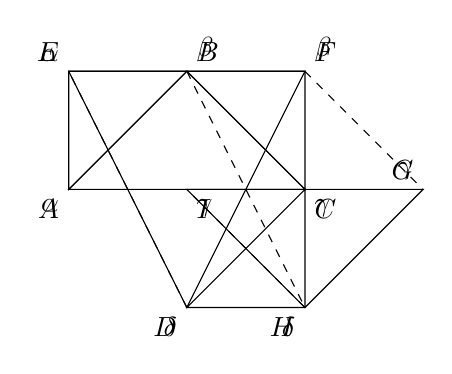
\begin{tikzpicture}[scale=1.5]

% Define coordinates
\coordinate (A) at (0,0);
\coordinate (B) at (1,1);
\coordinate (C) at (2,0);
\coordinate (D) at (1,-1);
\coordinate (E) at (0,1);
\coordinate (F) at (2,1);
\coordinate (G) at (3,0);
\coordinate (H) at (2,-1);
\coordinate (I) at (1,0);

% Draw the large triangle
\draw (A) -- (B) -- (C) -- cycle;
\draw (D) -- (E) -- (F) -- cycle;
\draw (G) -- (H) -- (I) -- cycle;

% Draw the smaller triangles
\draw (A) -- (E) -- (B) -- cycle;
\draw (B) -- (F) -- (C) -- cycle;
\draw (C) -- (H) -- (D) -- cycle;

% Label the points
\node at (A) [below left] {$A$};
\node at (B) [above right] {$B$};
\node at (C) [below right] {$C$};
\node at (D) [below left] {$D$};
\node at (E) [above left] {$E$};
\node at (F) [above right] {$F$};
\node at (G) [above left] {$G$};
\node at (H) [below left] {$H$};
\node at (I) [below right] {$I$};

% Draw the lines and labels for the planes
\draw[dashed] (A) -- (G);
\draw[dashed] (B) -- (H);
\draw[dashed] (C) -- (I);
\draw[dashed] (D) -- (E);
\draw[dashed] (F) -- (G);
\draw[dashed] (H) -- (I);

\node at (A) [below left] {$\alpha$};
\node at (B) [above right] {$\beta$};
\node at (C) [below right] {$\gamma$};
\node at (D) [below left] {$\delta$};
\node at (E) [above left] {$\alpha$};
\node at (F) [above right] {$\beta$};
\node at (G) [above left] {$\gamma$};
\node at (H) [below left] {$\delta$};
\node at (I) [below right] {$\gamma$};

\end{tikzpicture}

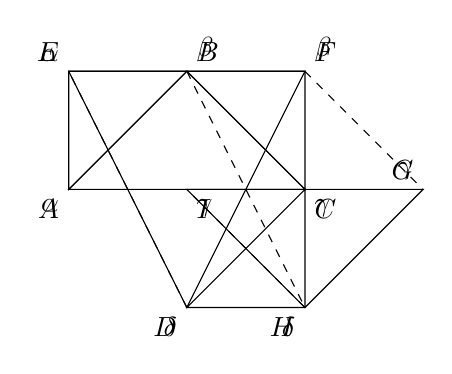
\begin{tikzpicture}[scale=1.5]

% Define coordinates
\coordinate (A) at (0,0);
\coordinate (B) at (1,1);
\coordinate (C) at (2,0);
\coordinate (D) at (1,-1);
\coordinate (E) at (0,1);
\coordinate (F) at (2,1);
\coordinate (G) at (3,0);
\coordinate (H) at (2,-1);
\coordinate (I) at (1,0);

% Draw the large triangle
\draw (A) -- (B) -- (C) -- cycle;
\draw (D) -- (E) -- (F) -- cycle;
\draw (G) -- (H) -- (I) -- cycle;

% Draw the smaller triangles
\draw (A) -- (E) -- (B) -- cycle;
\draw (B) -- (F) -- (C) -- cycle;
\draw (C) -- (H) -- (D) -- cycle;

% Label the points
\node at (A) [below left] {$A$};
\node at (B) [above right] {$B$};
\node at (C) [below right] {$C$};
\node at (D) [below left] {$D$};
\node at (E) [above left] {$E$};
\node at (F) [above right] {$F$};
\node at (G) [above left] {$G$};
\node at (H) [below left] {$H$};
\node at (I) [below right] {$I$};

% Draw the lines and labels for the planes
\draw[dashed] (A) -- (G);
\draw[dashed] (B) -- (H);
\draw[dashed] (C) -- (I);
\draw[dashed] (D) -- (E);
\draw[dashed] (F) -- (G);
\draw[dashed] (H) -- (I);

\node at (A) [below left] {$\alpha$};
\node at (B) [above right] {$\beta$};
\node at (C) [below right] {$\gamma$};
\node at (D) [below left] {$\delta$};
\node at (E) [above left] {$\alpha$};
\node at (F) [above right] {$\beta$};
\node at (G) [above left] {$\gamma$};
\node at (H) [below left] {$\delta$};
\node at (I) [below right] {$\gamma$};

\end{tikzpicture}

\end{document}